% Preamble
\documentclass[a4paper,12pt]{article}

\usepackage[osf]{mathpazo} % palatino
\usepackage{ms}            % load the template
\usepackage[round]{natbib} % author-year citations
\usepackage{graphicx}
\usepackage{parskip} 
\usepackage{caption}
\usepackage{subcaption}
\usepackage{textcomp} % for parts per mille symbol     
\pagenumbering{arabic}    
\linespread{1.66}

% Title page information
\title{Reconstructing the last known movements of one of Nature's giants}
% 90 characters max

\author{
  Clive N. Trueman$^{1}$, Andrew L. Jackson$^{2}$, Katharyn S. Chadwick$^{1}$,\\ 
  Ellen J. Coombs$^{3,4}$, Sarah Magozzi$^{1,5}$, Richard C. Sabin$^{3}$ \\
  and Natalie Cooper$^{3*}$
}
\date{}
\affiliation{\noindent{\footnotesize
  $^1$ Ocean and Earth Science, University of Southampton Waterfront Campus, Southampton, SO14 3ZH, UK.\\
  $^2$ School of Natural Sciences, Trinity College Dublin, Dublin 2, Ireland.\\
  $^3$ Department of Life Sciences, Natural History Museum London, Cromwell Road, London, SW7 5BD, UK.\\ 
  $^4$ Department of Earth Sciences, University College London, Gower Street, London, WC1E 6BT, UK.\\
  $^5$ Department of Geology and Geophysics, University of Utah, Salt Lake City, UT 84112-0102, USA.\\
  $*$Email address: natalie.cooper@nhm.ac.uk
}}

\vfill

%\runninghead{}
%\keywords{}
%}

% End of preamble

\begin{document}
\modulolinenumbers[1]   % Line numbering on every line

\mstitlepage

\parindent = 1.5em
\addtolength{\parskip}{.9em}

\raggedright

\section{Abstract}

The spatial ecology of rare, migratory oceanic mammals such as blue
whales (\textit{Balaenoptera musculus}) is difficult to study directly. 
Recent advances in satellite telemetry have improved our understanding of individual-level migratory behavior, but tags generally last only a few months, and cannot provide retrospective information. 
Incrementally-grown tissues provide an alternative means of reconstructing individual-level movements over long timescales, but inferring spatio-temporal information from biochemical tracers is challenging. 
Here we outline a new approach combining stable isotope analyses of incrementally-grown tissues with simulation models to test hypotheses relating to individual-level animal movements. 
We illustrate our new method by identifying the most likely multi-year movement history of a historic blue whale that stranded in 1891 and is now on display at the Natural History Museum, London. 
Our method unlocks movement information coded in biochemical compositions of incremental tissues including those housed in historic collections, and provides inferences that are complimentary to and comparable with tag-derived movement data.

\textbf{Keywords: carbon stable isotopes, movement models}

\section{Introduction}\label{background}

Migratory species pose a particular challenge for conservation practitioners because their effective conservation relies on protection at many, often distant, sites \citep{runge2014conserving}. 
Migratory species may also be particularly vulnerable to changes in climate or human use of the environment, as they are influenced by conditions in multiple locations across different parts of their life cycle \citep{robinson2009travelling}. 
Identifying threats to migratory species, understanding species responses to change and developing effective conservation measures all require information on the movements of individual animals over multiple years, ideally for both historic and present-day populations. 
With the development of electronic tagging technology, studies of the distributions of animals have largely shifted from infrequent observations of many individuals with limited or no information about individual movement behavior, to frequent observations of a few individuals, with detailed information about individual movement \citep{holdo2013inferring}. 
Despite the tremendous advances made using direct telemetry devices, tags are expensive, with a relatively high failure rate \citep{bailey2009behavioural,best2015tag,mate2007evolution}. 
Data on individual-level, multi-annual movements remain scarce, especially for rare, wide-ranging and long-lived marine species such as baleen whales (Mysticeti) \citep{ryan2013stable,hall2005stable,bailey2009behavioural}.

An alternative technique for investigating animal movements retrospectively is to use intrinsic biochemical information such as stable isotope compositions \citep{west2006stable,busquets2017estimating,hobson2008tracking}. 
Present-day populations can be studied with material collected in the field, while historic samples can be taken from museum collections; rich archives of behavioral information that are often under-utilised \citep{lister2011natural}. 
The stable isotope composition of animal tissues reflects the isotopic composition of diet at the time and place of ingestion, integrated over the timescale of tissue growth. 
A large literature describes the use of stable isotope markers to link the composition of a tissue to a geographic source at a single point in time \citep{hobson2008tracking}. 
Relating the isotopic compositions of marine animal tissues to the likely location of tissue growth is complicated by a lack of knowledge of spatial variations in the isotopic composition of diet (the isotopic baseline) \citep{west2006stable,mcmahon2015millennial}. 
This uncertainty is compounded when multiple samples are taken through time in the same individual, as temporal variation in the isotopic baseline must also be considered explicitly. 
Consequently, relatively little attention has been given to the potential to infer individual movement histories by reconstructing time series of multiple discrete origins from sequentially sampled incrementally-grown tissues 
% [trueman st john glew, Tokyo eel, darnaude, brennan?].

Recently, mechanistic models have been developed providing relatively accurate predictions of isotopic variability at high temporal and spatial resolution. 
These models can be coupled to Lagrangian or agent-based models of animal movement to predict isotopic compositions or trajectories expected to be recorded in animal tissues under differing movement scenarios. 
Here we illustrate the potential of this conceptual approach by assessing the relative likelihood of differing, plausible hypotheses of movement behavior for a single individual blue whale based on carbon isotope compositions sampled across a baleen plate.  
We draw on newly developed models predicting spatio-temporal variation in phytoplankton stable carbon isotope composition at global and monthly resolution \citep{magozzi2017using} (Figure S3), coupled to an agent-based model of whale movements (see Table S1; Figure S5). 
We specifically ask whether the isotopic profile observed in baleen can be simulated using agent based movement models informed by current understanding of animal movements and isotopic variability.

We apply our method a blue whales (\textit{Balaenoptera musculus}), the largest animal to have ever lived. 
Mysticete whales are characterized by the development of baleen, keratinous structures in the upper jaw used to filter food items from seawater. 
Baleen is ideal for stable isotope studies because keratin grows continuously through an individual's life, and once laid down it is metabolically inert \citep{best1996stable,hobson1998stable}. 
Baleen plates therefore offer a continuous isotopic record of behavior typically reflecting multiple years of life of an individual whale. 
Baleen is worn away at the tips over time, so a baleen plate reflects the most recent years of life, and rarely records an individual's entire lifespan. 
Among the mysticete whales, blue whales are a particularly attractive target for model-based isotope movement work as they have a consistent, low trophic level diet and feed continuously through the year, likely driven by high energetic costs of maintaining extreme muscle mass \citep{goldbogen2015}.

Similar to other large balaenopterid whales, blue whales are generally assumed to conduct annual migrations between high and low latitudes \citep{huckgaete2018}. 
As blue whales feed throughout the year to accommodate energetic costs, migration routes and feeding areas for blue whales are thought to be shaped by the year-round location of highly productive regions \citep{branch2007}. 
Recent studies tracking movements of individual blue whales primarily in the northeast Pacific have demonstrated high levels of among-individual variation in movement histories including suspending migration for opportunistic feeding and skipped migration (i.e. year round residency in either summer or winter
areas) \citep{busquets2017estimating}. 
However, most satellite deployments on blue whales report movement data for periods of time under six months \citep{heide2001new, silva2013north, bailey2009behavioural, lesage2017foraging, irvine2017quantifying}, and are unable to show individual movements between summer and winter feeding or breeding areas. 
The longest period of continuous monitoring via satellite tagging of an individual blue whale that we are aware of in the northeast Pacific is 504 days \citep{irvine2017quantifying} and in the North Atlantic is 177 days \citep{lesage2017foraging}.

The northeast Atlantic population of blue whales was the first large whale population to be systematically hunted with explosive harpoons, and while the population was probably relatively small before hunting, now around 1000 individuals are estimated to be in the northeast Atlantic in summer, mainly distributed around Iceland \citep{pike2009note}. 
The small population size and oceanic habit makes blue whale movements extremely hard to study. 
A combination of historic whaling data, observations, satellite tracks and acoustic monitoring suggests that blue whales in the northeast Atlantic also track regions of high production throughout the year, at least some whales wintering in the upwelling systems between Mauritania and the Cape Verde Islands \citep{baines2014upwellings}. 
Northward migration in the spring may occur along mid Atlantic corridors with peak sightings in the Azores around April-May \citep{silva2013north}. 
Summer feeding appears to occur in northerly latitudes around Iceland, and historically in the Norwegian and Barents Seas \citep{pike2009note}. 
Blue whales are frequently detected in waters to the west of the UK, with peak acoustic detections occurring between November and December, in southerly migrating animals \citep{reeves2004historical,baines2017autumn,charif2009acoustic,visser2011timing}.
To our knowledge one photographic identification has matched summer and winter locations of a single north-east Atlantic blue whale with sightings in Iceland and Mauritania \citep{poster}.

Inferences concerning movements of blue whales in general, and in the northeast Atlantic in particular, are therefore largely drawn from disparate information sources and rarely detail movements of individual animals over timescales of a year or more. 
It is particularly difficult to establish the degree of connectivity between summer and winter feeding areas, and the level of temporal consistency in movement behaviour within individuals. 
Information on historical movement patterns of individual blue whales is important for understanding the drivers of whale declines, and potential for human-whale conflicts as populations recover.

Here we aim to show that stable carbon isotope tracers can be used to test hypotheses about individual-level movement behavior, and can be applied to recent or historic archived samples. 
We apply our method to infer the most likely movement history for a blue whale stranding off the coast of Wexford Ireland in March 1891, and currently on display in the Natural History Museum, London (NHM). 
The NHM whale ``Hope'' is a female estimated to be a young adult at least 15 years at death. 
Baleen from the NHM whale therefore yields information about about a single blue whale living in the North Atlantic around the peak of industrial whaling.

\section{Materials and Methods}\label{methods}

\subsection{Stable isotope extractions from baleen}
\label{stable-isotope-extractions-from-baleen}

Baleen was collected from the Natural History Museum, London (specimen NHMUK.1892.3.1.1). 
The baleen plate was cleaned with ethanol to remove surface contaminants such as skin/gum or other lipids that can influence isotopic signals. 
{\raise.17ex\hbox{$\scriptstyle\sim$}}1mg samples of keratin powder were then collected from the plate using a hand-held drill and grinding bit. 
97 samples were taken at 1cm intervals, 0.5cm from the outer edge of the plate, starting at the proximal (gingival) section that contains the most recent tissue. 
Baleen grows at a constant rate, so the samples are equally spaced through time \citep{best1996stable}. 
Carbon and nitrogen isotope analysis was performed simultaneously via continuous-flow isotope ratio mass spectrometry at the University of Southampton SEAPORT Stable Isotope Ratio Mass Spectrometry Laboratory (Southampton, UK), using a Vario Isotope select elemental analyser, coupled to an Isoprime 100 isotope mass spectrometer. 
Replicates using internal laboratory standards (L-glutamic acid (C), Glutamic acid (CT standard), acetanilide and protein standard OAS) were used for quality control and calibration. 
C:N ratios for samples ranged from 3.28\text{\textperthousand} to 3.72\text{\textperthousand}, well within the acceptable theoretical range for pure keratin ($3.4\pm0.5$) allowing for comparison among samples \citep{hobson1998stable}. 
All data are available from the NHM Data Portal \citep{data-set} (https://doi.org/10.5519/0093278).

\subsection{Time calibrating stable isotope profiles}
\label{time-calibrating-stable-isotope-profiles}

Seasonal variations in isotopic gradients induce cyclical variations in the isotopic composition of baleen, the distance between cycles reflecting growth rates \citep{hobson1998stable,busquets2017estimating}. 
Clear periodicity was evident in $\delta^{15}$N values across the entire baleen plate, and in $\delta^{13}$C values in the youngest 70 - 18cm of the plate (behavioural phase two). 
We calculated isotopic periodicity within the NHM baleen sample using Fourier Transform analysis \citep{cardona2017temporal} (Figure S1), revealing a consistent growth rate of 13.5$cmy^{-1}$ which is remarkably similar to the mean isotope-derived baleen growth rates of $15.5 \pm 2.2cmy^{-1}$ estimated by \cite{busquets2017estimating}.  
Therefore we dated the youngest baleen sample as 1st March 1891, 24 days prior to the stranding date, 25th March 1891. 

\subsection{Baseline isotope comparisons}
\label{baseline-isotope-comparisons}

Isotope-enabled biogeochemical ocean models \citep{magozzi2017using,schmittner2016complementary} were used to characterize the isotopic composition of phytoplankton expected in different potential foraging grounds (Figure S3). 
Annual average \(\delta^{15}\)N POM (particulate organic matter) values were provided by C.J. Somes (\textit{pers.comm}) based on a 5\({}^{\circ}\) resolution biogeochemical model (Figure S3). 
\(\delta^{13}\)C POM values were simulated at 1\({}^{\circ}\) and monthly resolution using an isotopic extension to the NEMO-MEDUSA ocean biogeochemical model \citep{magozzi2017using,yool2013medusa}. 
Simulated \(\delta^{15}\)N POM values are relatively positive in the northeast Atlantic north of c. 60\({}^{\circ}\)N, and relatively negative in the central and southern North Atlantic. 
Annual average \(\delta^{13}\)C POM values largely vary with latitude, with more negative values in more northerly regions. 
In the central North Atlantic, \(\delta^{13}\)C POM values are relatively positive in the west, reflecting warm gulf stream waters (Figure S3). 
The isotopic composition of carbon in phytoplankton also varies through seasons as isotopic fractionation of carbon during photosynthesis is strongly influenced by sea surface temperature \citep{magozzi2017using,laws1995dependence}. 
Thus temporal variations in \(\delta^{13}\)C POM values are superimposed on latitudinal gradients. 
The scale and nature of temporal variation in \(\delta^{13}\)C POM values also varies with latitude, with higher latitude seas showing greater intra-annual variation in \(\delta^{13}\)C POM values linked to strongly seasonal phytoplankton growth dynamics.
The model simulations used are forced with decadal climatological data from 2000-2010 \citep{magozzi2017using}. 

The isotopic composition of phytoplankton is influenced by the release of fossil carbon with low \(\delta^{13}\)C values into the atmosphere (Suess effect) and the effect of increased concentrations of dissolved CO2 on isotopic fractionation during phytoplankton growth 
%(Young et al 2013)
, potentially complicating the application of a model trained on recent data to historic samples. 
Ocean basin scale spatio-temporal differences in \(\delta^{13}\)C values largely reflect relative differences in sea surface temperatures between trophic, temperate and arctic waters and over seasons, and we assume that any regional variation in isotopic effects due to CO\textsubscript{2}-influenced changes in phytoplankton composition and growth rate are minor compared to latitudinal and seasonal variations in \(\delta^{13}\)C POM values. 
We do not draw inferences about location from absolute \(\delta^{13}\)C values and thus the reduction in oceanic \(\delta^{13}\)C POM values does not directly influence inferences about location or movement.  
We are therefore confident that the \cite{magozzi2017using} model can be applied to interpret historic baleen isotope data at least at ocean-basin scale spatial resolution.

We used \(\delta^{13}\)C POM values modeled at monthly resolution to simulate the isotopic expression of phytoplankton expected to be encountered by whales exhibiting differing movement behaviours. 
The stable isotope compositions of keratin at a given point in the baleen will reflect the stable isotope compositions of the krill it was feeding on in the weeks prior to keratin growth. 
Assimilation of carbon into krill tissues will dampen the temporal variability seen in POM, effectively producing a temporal average over the timescale of isotopic turnover within krill. 
We estimate turnover to be complete between two and four months and therefore we resampled the \(\delta^{13}\)C POM values in each one degree cell to reflect an average of isotopic compositions in phytoplankton in the two months prior to the sampling date. 
Average values were weighted according to the proportional plankton biomass estimated for each month. 
Carbon isotope values are also likely to be fractionated during transfer from plankton to krill as \textsuperscript{12}C is preferentially lost through respiration. 
The degree of such trophic fractionation is unclear, however and as we do not draw interpretations based on absolute \(\delta^{13}\)C values, rather on the relative \(\delta^{13}\)C values across the length of the baleen plate, we do not need to quantify this trophic enrichment effect. 
We assume that carbon available for synthesis of keratin is drawn from carbon released by respiration of diet captured opportunistically throughout the year \citep{baines2017autumn,silva2013north,visser2011timing,busquets2017estimating, lesage2017foraging, bailey2009behavioural, branch2007, huckgaete2018}.

\subsection{Agent-based whale movement model}
\label{agent-based-whale-movement-model}

We simulated the likely isotopic expression associated with different movement behaviours by building an agent-based movement model within the R coding environment, where movement behavior is influenced by sea surface temperature and phytoplankton biomass estimates provided by NEMO-MEDUSA \citep{yool2013medusa}, and bathymetry from the General Bathymetric Chart of the Oceans (GEBCO) \citep{bathy}, extracted via the marmap package in R \citep{marmap} (Figure S5).
% check figure S5

We simulated whale movements with the likelihood, direction, and extent of movement influenced by behavioral state, sea surface temperature, water depth, and phytoplankton concentration (as a proxy for zooplankton food availability).
Movement was coded as a set of probabilistic rules, informed by the literature on blue whale behavior (e.g. \citep{handbook}).
All terms were expressed as probability distributions, yielding multiple potential movement tracks.

In the models, the likelihood of moving, direction (north, south, east, west, northeast, northwest, southeast, or southwest) and linear distance of movement are all influenced by the following. 
(i) Behavioural state (migrating north, migrating south, or foraging, fixed according to month as defined by the operator).
Directly, northerly migrations were coded to occur in spring, and southerly migrations in autumn.
Foraging was possible at any time of year, and was triggered when whales encountered high concentrations of plankton.
(ii) Sea surface temperature \citep{yool2013medusa} ($^{\circ}$C). 
When migrating north, whales were more likely to move towards lower temperatures provided they were above the minimum temperature threshold (3$^{\circ}$C); whereas whales migrating south sought warmer waters.  
(iii) Water depth (m; from the General Bathymetric Chart of the Oceans (GEBCO) global bathymetry dataset\citep{bathy}, extracted via the marmap package in R \citep{marmap}). 
Whales were less likely to move into waters less than 400m deep, and increasingly unlikely to move into even shallower waters. 
(iv) Phytoplankton concentration ($mmolNm^{-3}$, for combined diatom and non-diatom communities \citep{yool2013medusa}). 
This was included as a proxy for zooplankton food availability. 
Whales are more likely to move towards (or remain within) areas of high phytoplankton density, particularly during the foraging behavioural state. 
At each daily step, the probability of movement, movement direction and distance traveled are sampled from probability distributions to allow individual variation.

Initial boundary conditions are defined with a maximum temperature of 25$^{\circ}$C and minimum temperature of 3$^{\circ}$C. 
The likelihood of movement (i.e. whether to move or not from the current location) is sampled from a binomial distribution with the probability of movement influenced by behavioural state and external conditions. 
The maximum daily movement distance permitted in each behavioural state is defined as a random sample of a Gaussian distribution with specified mean and standard deviation (see Table S1).

The agent-based mode provides daily location data points which are then used to extract time averaged \(\delta^{13}\)C values from the isotopic extension to the NEMO-MEDUSA model and assembled to build simulated isotopic profiles across baleen plates.
We created experimental movement models by manipulating the relative duration of the foraging and migratory behavioural states to produce simulated records of isotopic composition of carbon in baleen expected under differing movement trajectories. 
We simulated the isotopic expression expected for (a) residency in each known hotspot for blue whale sightings or historic hunting grounds in the North Atlantic (Norwegian/Barents Sea, West Ireland, Canaries/Azores and Mid Atlantic Ridge, and the Cape Verde/Mauritanian upwelling area \citep{mcdonald2006biogeographic,reilly2008balaenoptera,sigurjonsson1995life}; Figure S4); (b) seasonal migration between high sub-Arctic latitudes and temperate latitudes around the British Isles and (c) seasonal migration between high latitudes and subtropical latitudes.

We simulated two years of residency 30 times for each residency hotspot (Figure S4). 
We simulated seven years of whale movements 1200 times, then excluded simulations where the virtual whale stranded before reaching the 3019 days of the baleen record, leaving 1049 simulations. 
We then compared the simulated stable isotope profiles (Figure \ref{fig3}) to the profile measured in the blue whale baleen (Figure \ref{fig1}) with simple linear regressions.

For a full description of the model and its parameters see Figure S5 and Table S1. 
R code for all analyses is available from GitHub (https://github.com/nhcooper123/blue-whale-bes; \citep{github})

\section{Results}

\subsection{Baleen stable isotope profiles}
The baleen plate yielded 97 discrete samples of baleen.
\(\delta^{15}\)N values measured in the baleen plate display regular cyclical fluctuations throughout the length of the plate. Fourier analysis (periodogram function in the R package TSA \citep{Chan:2012aa}) revealed a strong periodic repetition with a 13.3cm periodicity, with a mean spacing of 13.5cm, assumed to represent annual periodicity. 
Therefore, given the date of stranding (25th March 1891), and estimated baleen growth rates of 13.5cm y$^{-1}$, we reconstructed a timeline for \(\delta^{13}\)C and \(\delta^{15}\)N fluctuations in the baleen over seven full years of the whale’s life (early 1884 - spring 1891). 

\(\delta^{13}\)C values are relatively high and constant in the oldest (most distal) 35cm of the baleen plate, associated with a weakening of the periodic fluctuation seen in \(\delta^{15}\)N values, and an overall reduction in \(\delta^{15}\)N values. 
This is followed by a clear change towards repeated fluctuations in \(\delta^{13}\)C values in the middle 50cm of the baleen plate, with a similar periodicity of 13.5cm (Figure \ref{fig1}). 
A second, distinct change in the pattern of \(\delta^{13}\)C values along the baleen plate occurs at around 84cm from the distal end, with a transition to uniform, relatively low \(\delta^{13}\)C values followed by an abrupt transition to positive \(\delta^{13}\)C values and a decline in \(\delta^{13}\)C values in the most recent (most gingival) 3cm of the record.

The \(\delta^{13}\)C and \(\delta^{15}\)N profiles therefore divide the isotopic record into two distinct phases that we assume reflect changes in the whale’s behaviour. 
In behavioural phase one (from the start of the record to spring 1886), we find relatively stable, elevated \(\delta^{13}\)C values, and relatively low \(\delta^{15}\)N values (Figure \ref{fig1}; Figures S1 and S2). 
In behavioural phase two (summer 1886 to spring 1890) \(\delta^{15}\)N values are relatively high and \(\delta^{13}\)C values are relatively low with coincident cyclical fluctuations in both \(\delta^{13}\)C and \(\delta^{15}\)N values.
In the last year of life the cyclical pattern is disrupted, with constant low \(\delta^{13}\)C values for approximately six months in the first half of 1890, before a rapid switch to relatively high \(\delta^{13}\)C values in the second half of 1890. 
The final three months of the record show a progressive fall in \(\delta^{13}\)C values (Figure \ref{fig1}; Figures S1 and S2). 
Cross-correlation analysis demonstrates a strong negative covariance between \(\delta^{13}\)C and \(\delta^{15}\)N values within behavioural phase two (Figure S2), but no relationship between \(\delta^{13}\)C and \(\delta^{15}\)N values exists during behavioural phase one.

% figure 1
\begin{figure}
  \centering
  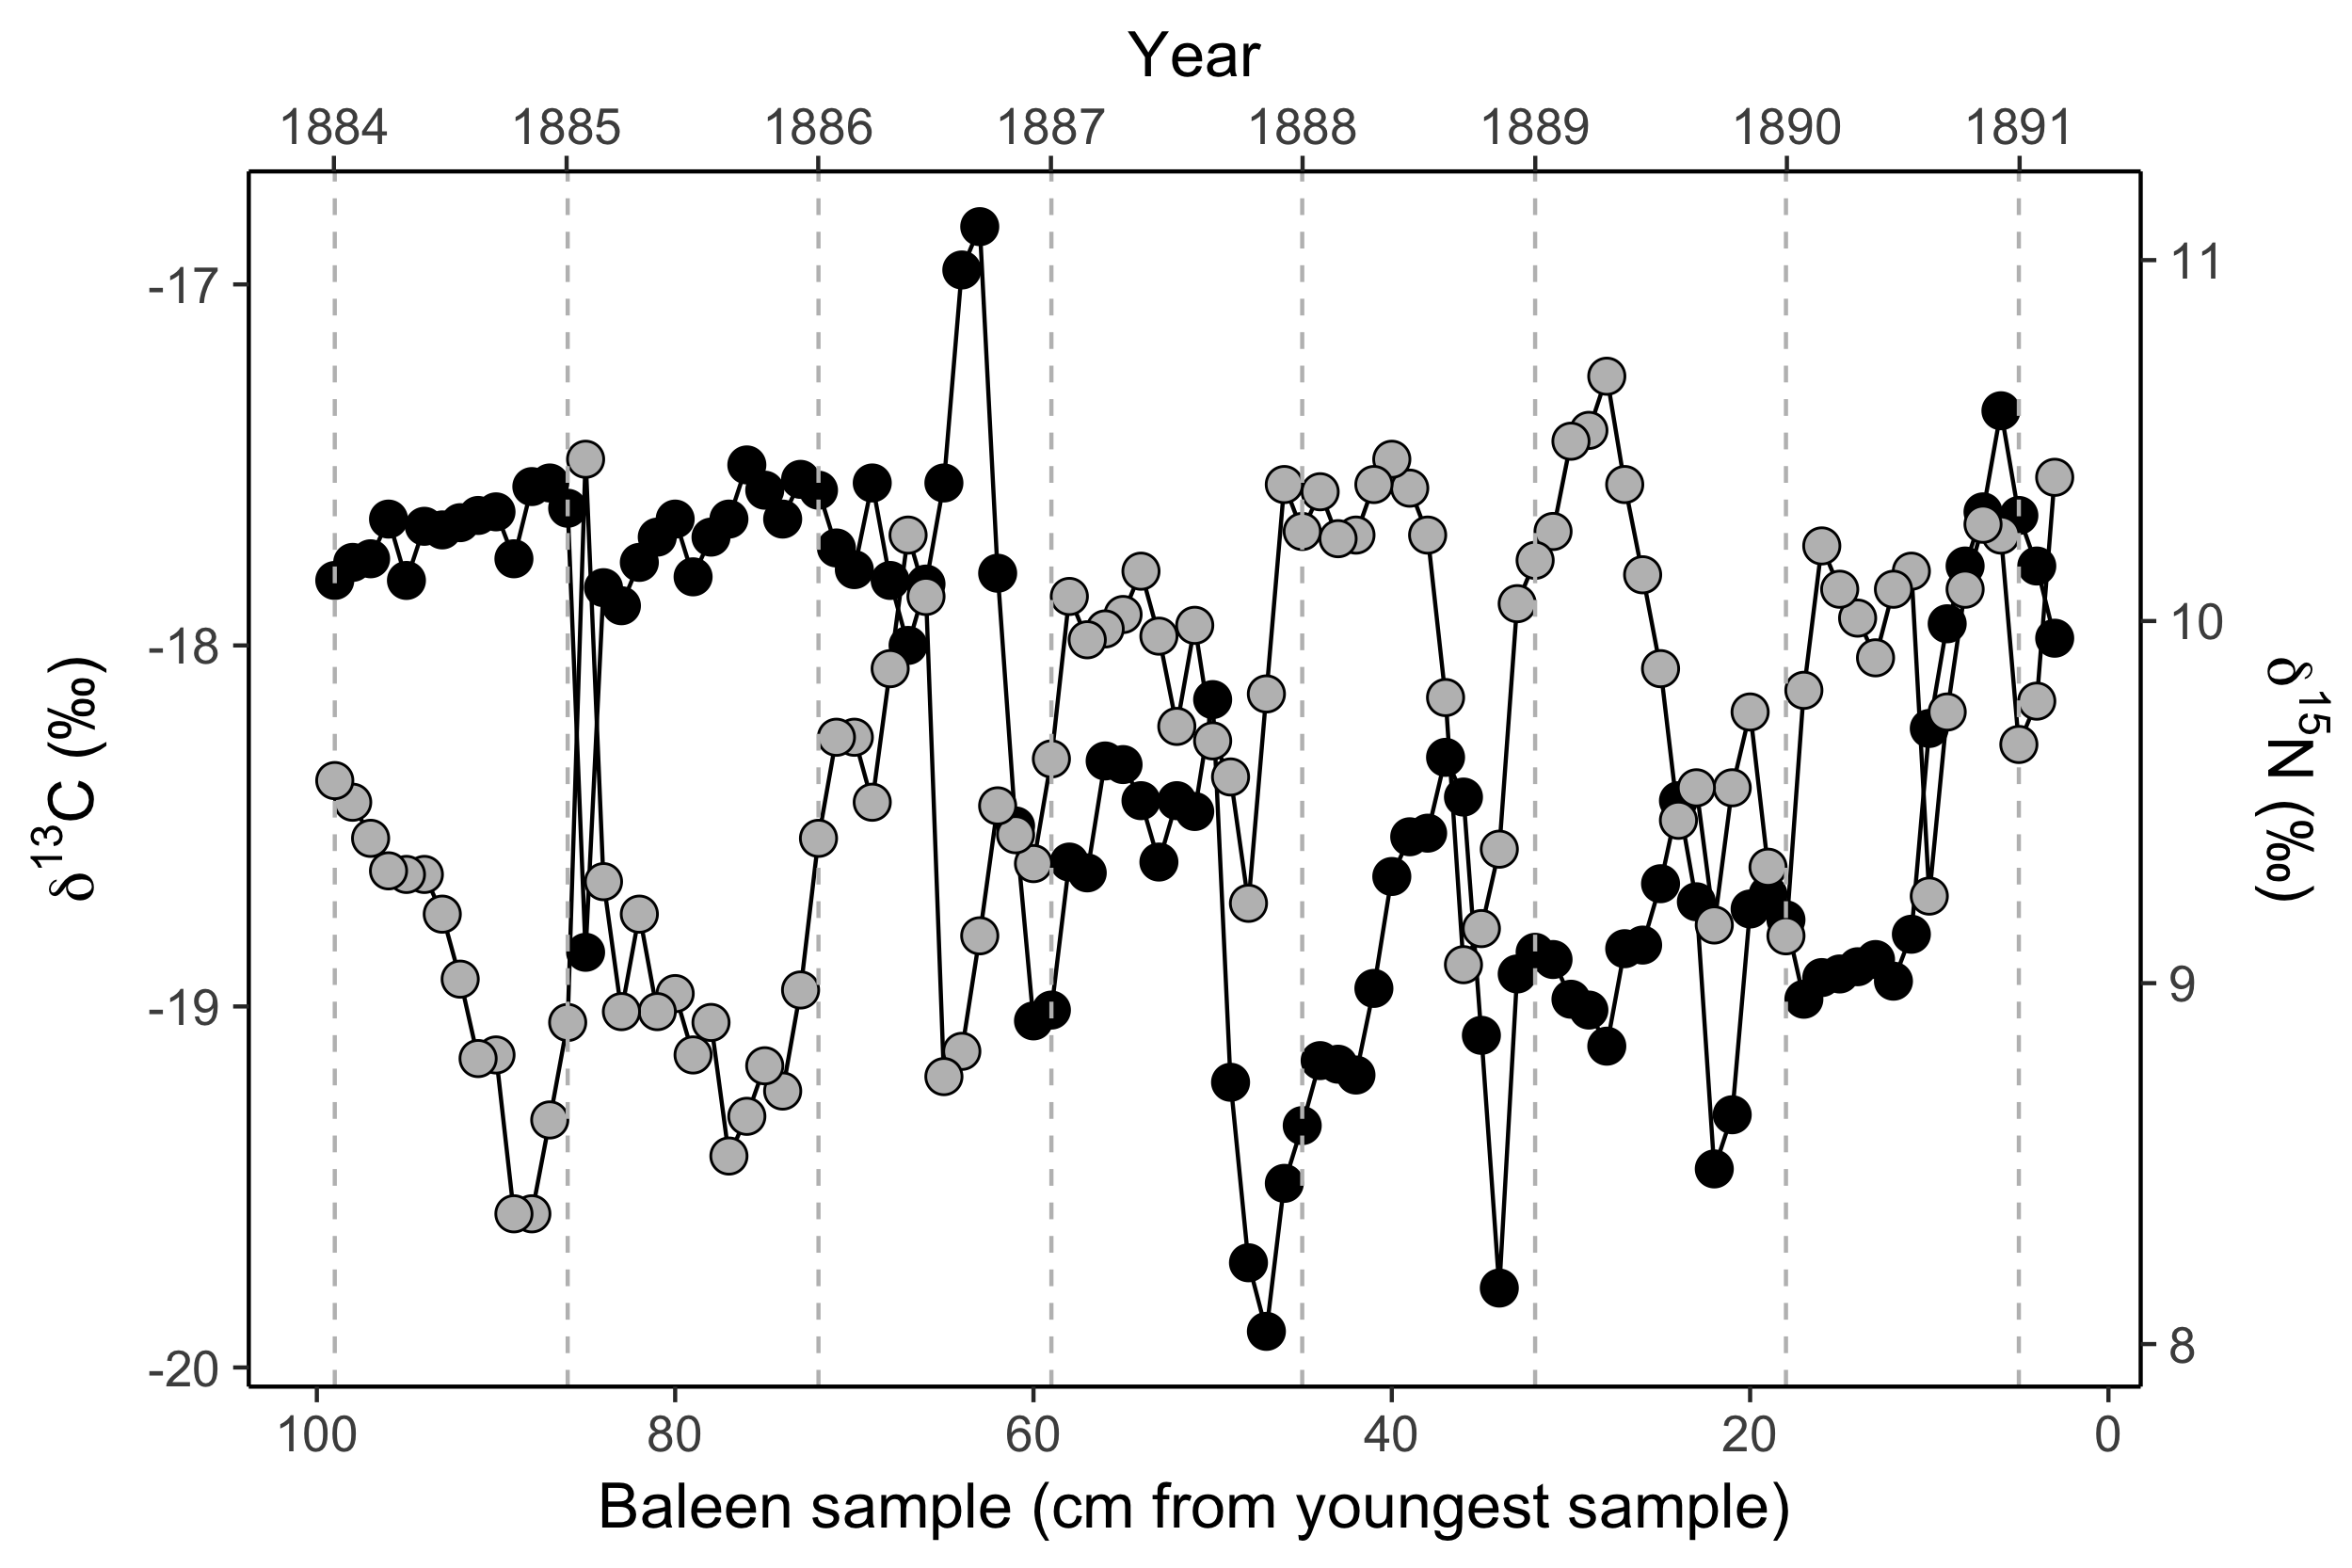
\includegraphics[width = \linewidth]{figures/Figure-1-raw-dC-dN-data.png}
  \caption{Variation in stable isotope values in the NHM blue whale, expressed as $\delta^{13}$C (black circles, left y-axis) and $\delta^{15}$N (grey circles, right y-axis). Samples were taken longitudinally through the baleen plate (n = 97 samples from a single baleen plate for both isotopes). There is strong annual periodicity and cross-correlation (Figures S1 and S2) in both isotopes. The approximate relationship to years assuming a growth rate of 13.5cm y$^{-1}$ is shown on the upper x-axis, and year boundaries are indicated by vertical dotted grey lines.}
  \label{fig1}
\end{figure}

\subsection{Agent-based whale movement model}

% figure 2
\begin{figure}
 \centering
 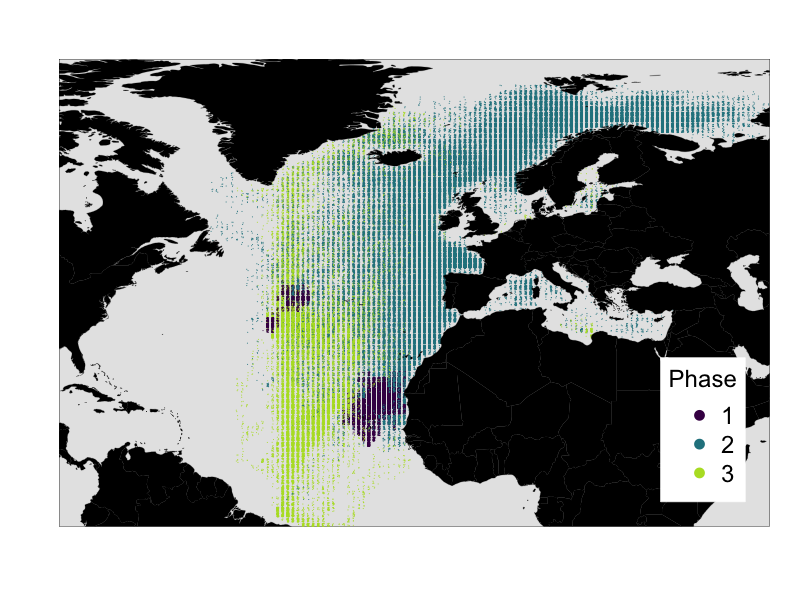
\includegraphics[width = \linewidth]{figures/Figure-2-points.png}
  \caption{Simulated locations of the whale taken from the top 10\% best fitting migratory movement models. 
  Colours reflect the behavioural phase. 
  Phase one is early 1884 to spring 1886, phase two is summer 1886 to spring 1890, and phase three is spring 1890 to spring 1891.}
  \label{fig2}
\end{figure}

We initially simulated temporal variations in baseline (phytoplankton) isotopic compositions that would be encountered by whales foraging within broad geographic regions (west UK/Irish shelf, Norwegian/Barents Sea, Canaries/west Azores, Mid-Atlantic ridge, Cape Verde/Mauritanian upwelling area; Figure S4). 
Strong seasonal dynamics in $\delta^{13}$C values are evident in all northerly regions, characterized by a rapid increase to annual maximum $\delta^{13}$C values associated with the onset of the spring phytoplankton bloom, followed by a more gradual decline in $\delta^{13}$C values towards minima in winter conditions (Figure S4). 
In temperate latitudes around the British Isles, seasonal dynamic cycles are present, but dampened (Figure S4), whereas in sub-tropical regions exemplified by the Canaries, Azores and particularly Mauritanian upwelling areas, $\delta^{13}$C values are relatively high and constant throughout the year (Figure S4).

Adding seasonal north-south migrations within mid-high latitude regions to foraging models yielded simulated profiles with regular isotopic fluctuations of relatively high amplitude reflecting $\delta^{13}$C minima preceding the June bloom (Figure S4, Figure \ref{fig1}). 

\subsection{Comparing the observed baleen isotopic profile to the model}
In the measured profile, behavioural phase one is characterised by relatively high and constant $\delta^{13}$C values.
$\delta^{15}$N values in this phase are relatively low and the isotopic cyclicity is absent (Figure S1).  
The relatively high and seasonally-invariant $\delta^{13}$C values seen during behavioural phase one are only found in subtropical areas of the North Atlantic. 
Our simulations identify a range of possible locations for the whale (Figure \ref{fig2}), although areas around the Mauritanian coast and Cape Verde Islands, a known current and historic winter feeding area for blue whales \citep{baines2014upwellings,reeves2004historical}, and potentially to the west of the Azores (Figure \ref{fig2}), most closely match the measured profile.
Temporal dynamics in $\delta^{13}$C values observed in the measured baleen during phase two cannot be reproduced in the simulated resident whales (Figure \ref{fig3}, Figure S4).
During behavioral phase two, the observed low $\delta^{13}$C values imply foraging in colder, more northerly latitudes. 
The pronounced cyclical variations in $\delta^{13}$C values observed during behavioral phase two could reflect either the isotopic expression of the spring phytoplankton bloom in northern waters \citep{magozzi2017using}, latitudinal migrations, or a combination of both. 
Accordingly we modeled whale movements allowing three years of residency in warm waters of the Azores or Cape Verde/Mauritania region followed by a further 3.5 years of seasonal north-south migration in the northeast northern Atlantic. 
We simulated 1200 individual movement patterns, then excluded simulations where the virtual whale stranded before reaching the 3019 days represented in the baleen.
We then compared the remaining 1049 simulations and the resulting simulated baleen $\delta^{13}$C records, to the measured records with simple linear regressions. 
Simulated baleen $\delta^{13}$C profiles produce a good fit to measured profiles, the median r\textsuperscript{2} value across 1049 simulated profiles was 0.31, and the maximum was 0.65 (Figure S6). 
The top 10\% best fitting simulated profiles are shown in Figure \ref{fig2}. 
Best fitting models predict residency in the Cape Verde region in behavioral phase one. Behavioral phase two is best simulated by seasonal migrations between summer foraging in northern areas (e.g. Norwegian Sea/Barents Sea/Iceland region), and winter foraging in a broad region between the UK and more southerly, subtropical waters. Better-fitting models in general were those predicting a greater latitudinal foraging range, and foraging in more northerly waters (Figures S7 and S8). 
Best-fit model distributions are largely consistent with current understanding of blue whale distributions in the northeast Atlantic \citep{reeves2004historical,baines2014upwellings,baines2017autumn,reeves2004historical} with perhaps greater importance of winter foraging in temperate regions (Figure \ref{fig4}).

% figure 3
\begin{figure}
 \centering
  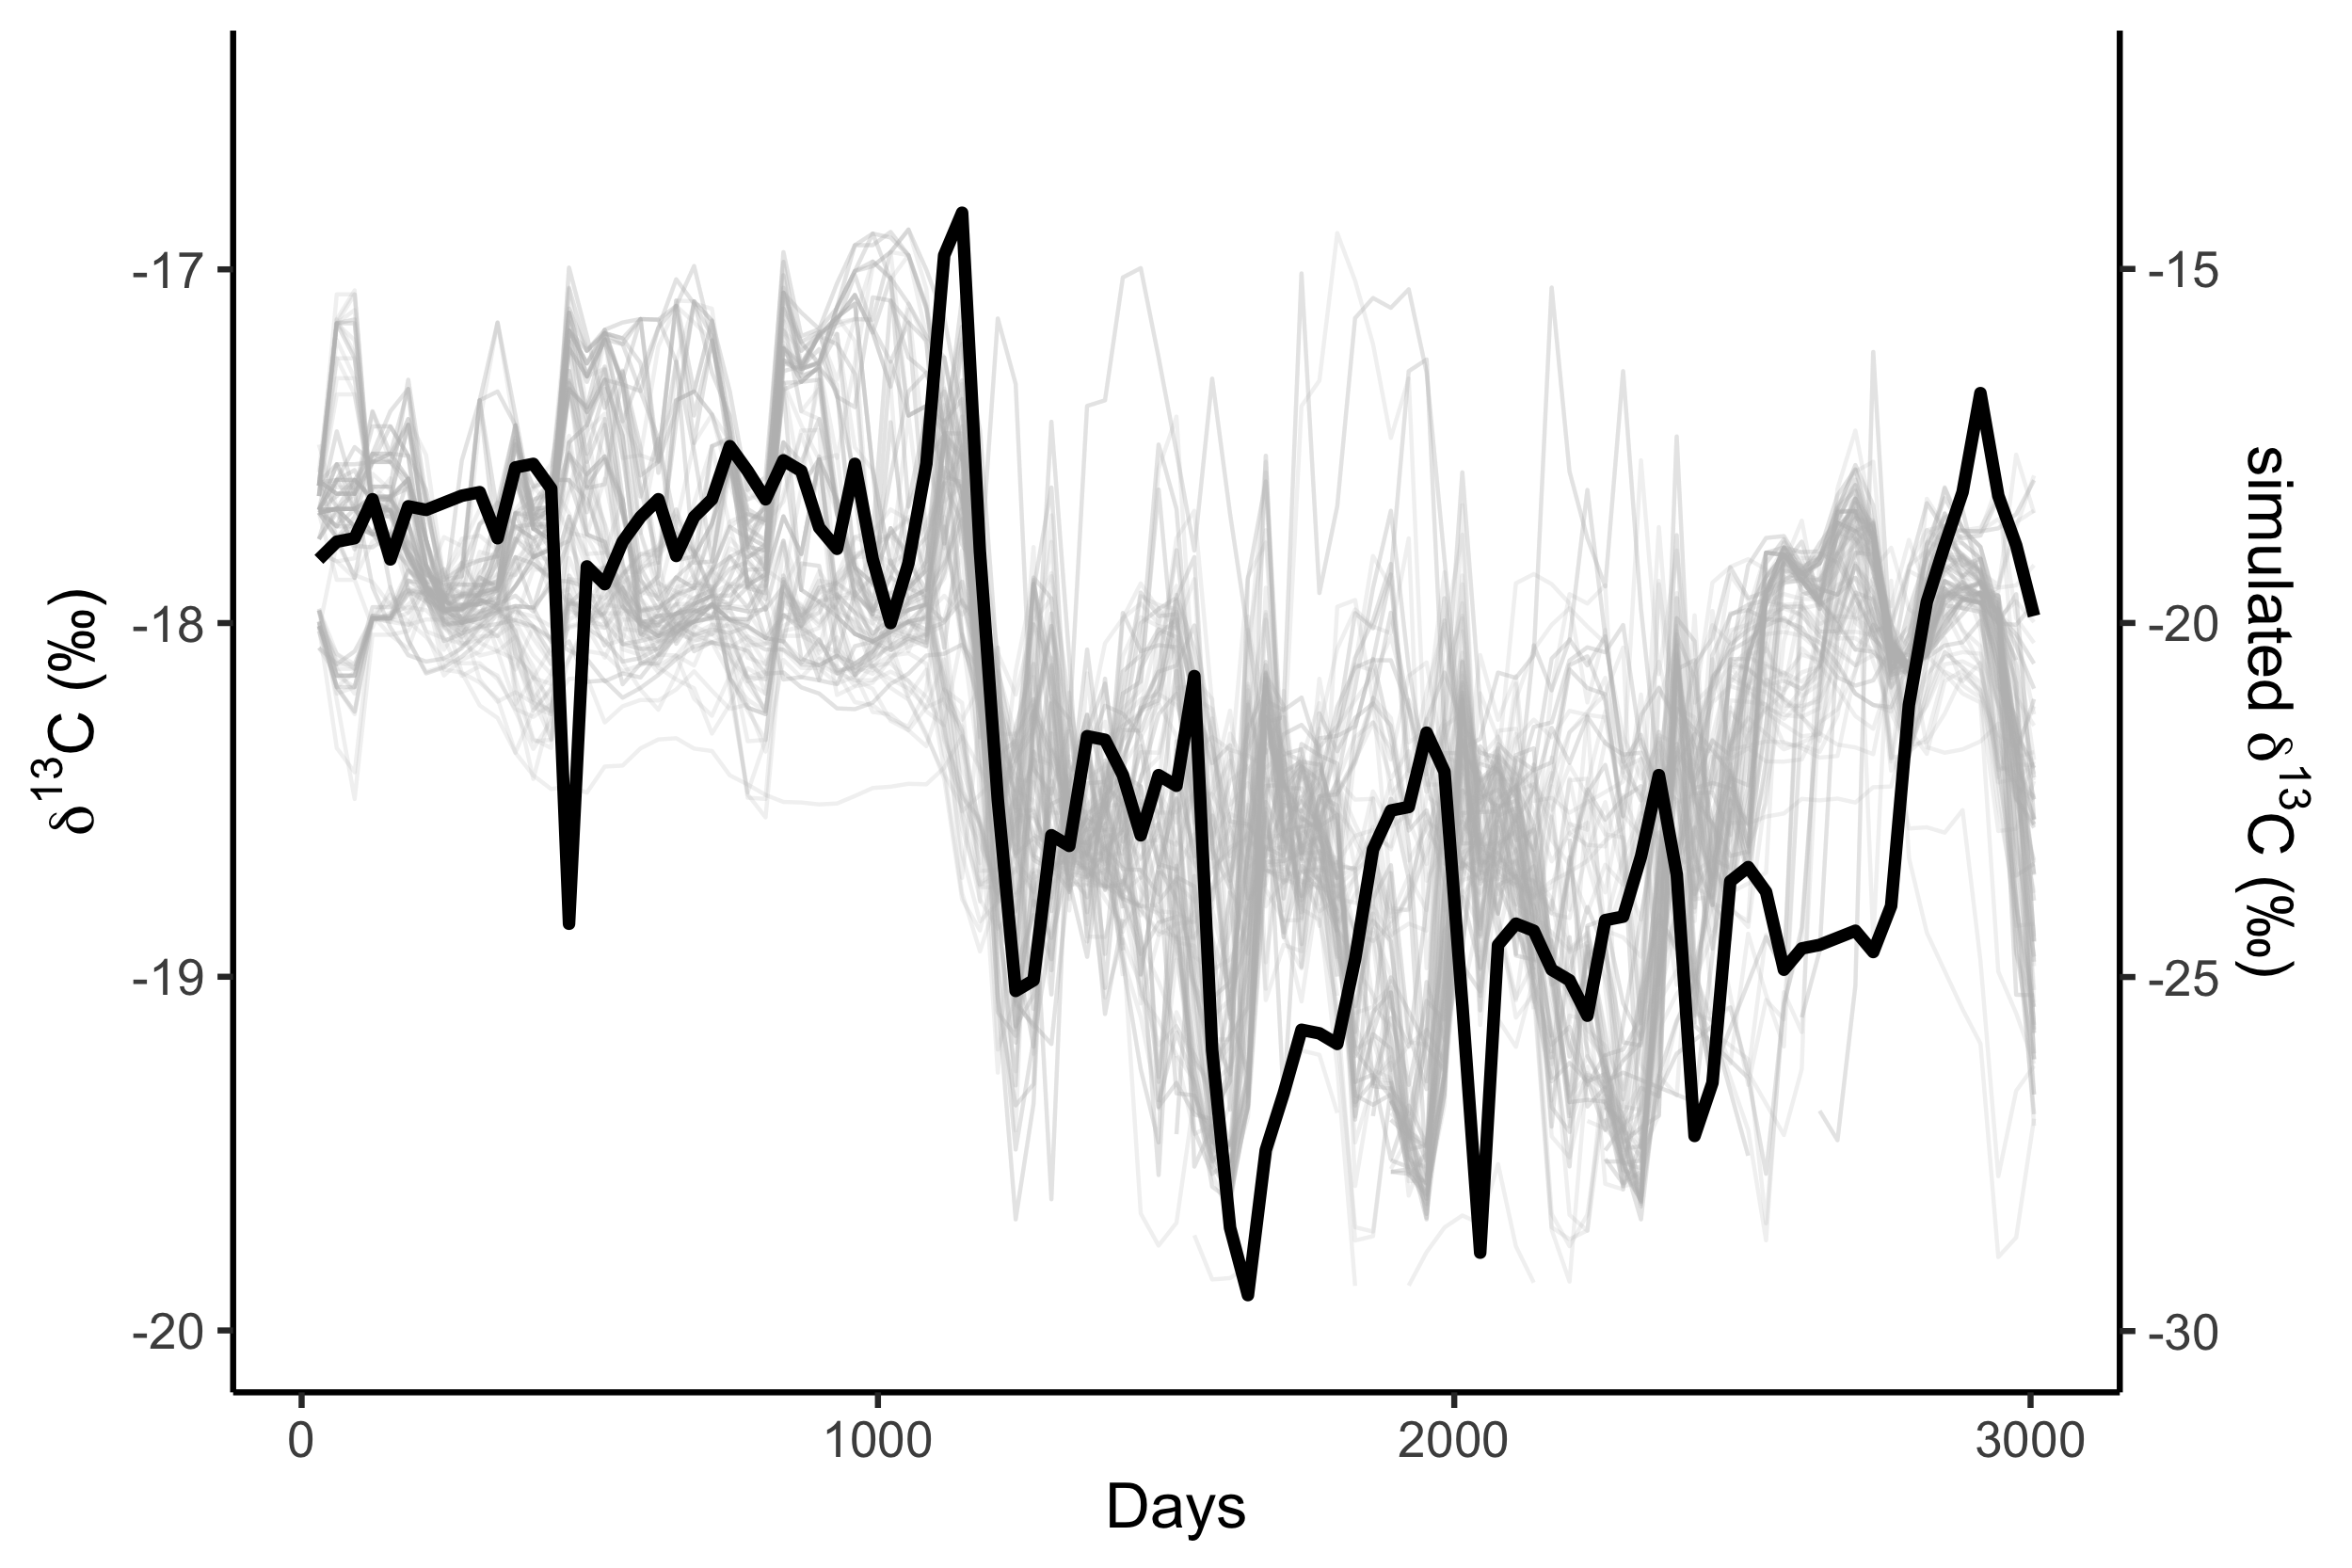
\includegraphics[width = \linewidth]{figures/Figure-3-blue-sims.png}
  \caption{Correlations among simulated $\delta^{13}$C from the top 10\% best fitting migratory movement models (grey lines, right hand y-axis) and $\delta^{13}$C from baleen (black line, left hand y-axis; see Figure \ref{fig1}). 
  Simulated $\delta^{13}$C values are six month moving average values for the time series of simulated plankton $\delta^{13}$C values in that location, reflecting temporal integration of phytoplankton $\delta^{13}$C values within the food chain before ingestion by the whale as krill. 
  The end points of the simulations and empirical data have been aligned to coincide.
}
  \label{fig3}
\end{figure}


% figure 4
\begin{figure}
 \centering
  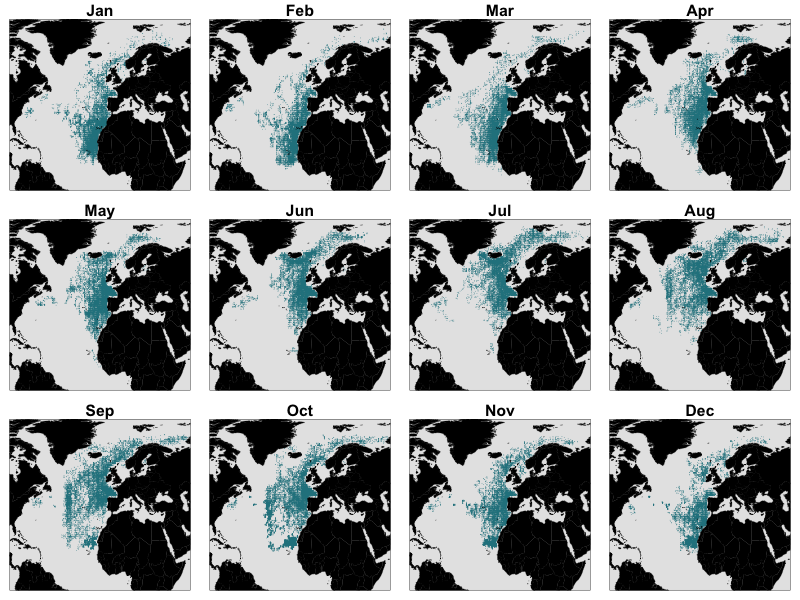
\includegraphics[width = \linewidth]{figures/Figure-4-monthly.png}
  \caption{Simulated locations by month taken from the top 10\% best fitting migratory movement models for behavioural phase two (summer 1886 to spring 1890) only.}
  \label{fig4}
\end{figure}

\subsection{Discussion}
Long-term, multi-annual data on the movement patterns and reproductive ecology of individual migratory marine animals are scarce, and stable isotope data provide a promising source of additional indirect information regarding spatio-temporal behavior, but interpreting such profiles is difficult, particularly in marine environments, because of unknown temporal and spatial variation in isotopic baselines.

Here we show how simulation models can be used to infer the isotopic expression expected from particular spatio-temporal foraging behaviours, and thus can be used used to interpret measured isotope data. 
We tested whether the isotopic variations observed across 6-7 years of growth of a baleen plate in a single blue whale could be simulated by agent based models coding for year round residency in known hotspots. 
We found that the isotopic record measured during behavioural phase one could be simulated through year round residency in relatively warm, subtropical waters with limited seasonal phytoplankton blooms. 
The measured profile is therefore consistent with residency in warm sub-tropical waters for at least one full year.
Hope was estimated to be at least 15 years old when she died (based on vertebral epiphyseal fusion; R.C. Sabin pers.comm), so was probably older than 10 years old, and therefore sexually mature, during this period.

The measured isotopic variations seen in behavioural phase two, characterized by repeated high amplitude cycles in $\delta^{13}$C values were best matched by movement models coded for annual latitudinal migrations with best fitting models predicting greater latitudinal foraging ranges. 
We therefore infer that Hope conducted at least three annual latitudinal migration cycles.
The last 500 days of Hope's life are difficult to simulate. 
Beginning in the winter of 1889/1890, the observed $\delta^{13}$C values are relatively low, and remain constant for c.4-6 months, before increasing rapidly in the second half of 1890. Low $\delta^{13}$C values are found in northern waters, but these areas also show large temporal fluctuations in $\delta^{13}$Cplk values (Figure S4), and the observed values cannot be simulated purely from movements within the known geographic range. 
We tentatively suggest that the $\delta^{13}$C record in the last period of life may be associated with pregnancy and calf rearing. 
Constant, low $\delta^{13}$C values may reflect later metabolic release of carbon reserves assimilated from northern latitudes (i.e. a period of time with limited opportunistic foraging). 
After c.4-6 months the whale began ingesting food with relatively high $\delta^{13}$C values, indicating feeding in low latitude waters, shortly followed by a final northward migration. 
Blue whales have a 10-12 month gestation period, with calving occurring in subtropical waters, and calves are weaned after 6-7 months \citep{handbook}.
We therefore infer a movement chronology reflecting three years of uninterrupted annual latitudinal migrations leading to pregnancy in the year 1889 and birth in the winter of 1889/1890. 
Following birth, we infer a period of c.4-6 months of residency in sub-tropical waters where the whale was sustained largely from stored lipid reserves, which we interpret as reflecting weaning. 
Subsequently we propose that the whale had a short period of feeding in sub-tropical waters in the second half of 1890 potentially during a final northward migration and eventual stranding during the return to northern feeding grounds in early 1891.

Whaling was an intense pressure for blue whales during the period we are analysing. 
Before whaling in the North Atlantic began in 1868 \citep{reilly2008balaenoptera}, there were and estimated 10,000-15,000 blue whales in the region \citep{sigurjonsson1995life}. 
In the early 20th century, fisheries moved outside the area because stocks were so depleted \citep{reilly2008balaenoptera}; during this period over 12,000 blue whales were landed \citep{sigurjonsson1995life}.
The NHM blue whale was thus an individual from a species at the brink of local extinction, potentially representing more than 0.1\% of the entire population of blue whales in the northeast Atlantic. 
Inferring spatio-temporal distributions of populations from high density observations of a few individuals (or, in this case one individual) will always be problematic, but the predictive power associated with linking a tracked individual to the population distribution increases when the tracked animal has a strong preference for specific habitats and there is a patchy (clumped) distribution of those habitats \citep{holdo2013inferring}. 
In the case of blue whales, the primary driver influencing seasonal movements is assumed to be the seasonally variable distribution of food resources between high and low latitudes. 
As blue whales have a relatively restricted diet that shows highly predictable spatio-temporal differences in abundance at least on ocean basin scales, we argue that the seasonal latitudinal migrations inferred during behavioural phase two are likely to be common movement traits within North Atlantic blue whales. 
This inference of course requires testing with additional isotopic records from individual whales, observational sightings data and multi-year satellite tracking records. 
Developing an understanding of the nature and plasticity of individual level movements in populations of blue (and other mysticete) whales would aid management decision making in the conservation of this endangered species \citep{irvine2017quantifying}.

\subsection{Conclusion}
Temporal variations in stable isotope compositions of incrementally grown tissues offer a potentially valuable record of movement in migratory organisms, but interpreting such profiles is extremely difficult, particularly in marine environments. 
Here we show how a simulation framework can be used to help interpret measured data through in silico experimentation. By varying parameters of agent-based movement models coupled to models predicting temporal and spatial variation in plankton carbon isotope data we identify combinations of movement behaviours producing simulated baleen isotope records that are most consistent with measured data.
Measured tracks can only be replicated by combination of residency and seasonal migration with latitudinal migrations limited to the last four years of simulations. 
Our results confirm that sequential sampling of stable isotope compositions in whale baleen, combined with simulation modeling can yield plausible inferences of individual whale movements that are consistent with assumed movement behaviours. 
Our movement simulation modeling removes a long-standing limitation in stable isotope ecology, and can be applied to stable isotope records from any incrementally-grown tissue to estimate most likely individual movement behaviors over multiple years. 
By unlocking information contained in incrementally-grown tissues we hope that a more detailed picture of individual movement behaviour in modern and historic mysticete whales (and other animals) can be developed.

\section{Acknowledgments}\label{acknowledgments}
This work was funded by the British Ecological Society (grant: 5771/6815). 
We thank C.J. Somes for providing $\delta^{15}$N POM data, Bastian Hambach and Megan Spencer at the University of Southampton SEAPORT isotope laboratory for assistance with stable isotope analyses, and Andrew Yool for allowing us to use and share NEMO-MEDUSA outputs.

% References
\bibliographystyle{refs}
%\bibliographystyle{authordate1}
\bibliography{blue-whale-abbreviations}

\subsection{Data Code and Materials}\label{data-code-and-materials}
Data are available from the NHM Data Portal (https://doi.org/10.5519/0093278). 
R code is available from GitHub (https://github.com/nhcooper123/blue-whale-bes)(Zenodo DOI 10.5281/zenodo.2542777).

\end{document}
